\achapter{19}{Path Connected Spaces}\label{sec:Path_connected_topology}


\vspace*{-17 pt}
\framebox{
\parbox{\dimexpr\linewidth-3\fboxsep-3\fboxrule}
{\begin{fqs}
\item What is a path in a topological space?
\item What is a path connected subset of a topological space?
\item What is a path connected component of a topological space?
\item What is a locally path connected space?
\item What connections are there between connected spaces and path connected spaces?
\end{fqs}}}

\vspace*{13 pt}

\csection{Introduction}

We defined connectedness in terms of separability by open sets. There are other ways to look at connectedness. For example, the subset $(0,1)$ is connected in $\R$ because we can draw a line segment (which we will call a \emph{path}) between any two points in $(0,1)$ and remain in the set $(0,1)$. So we might alternatively consider a topological space to be connected if there is always a path from one point in the spaced to another. Although this is a new notion of connectedness, we will see that path connectedness and connectedness are related.
 
Intuitively, a space is path connected if there is a path in the space between any two points in the space. To formalize this idea, we need to define what we mean by a path. Simply put, a path is a continuous curve between two points. We can therefore define a path as a continuous function.

\begin{definition} Let $X$ be a topological space. A \textbf{path}\index{path} from point $a$ to point $b$ in $X$ is a continuous function $p: [0,1] \to X$ such that $p(0) = a$ and $p(1)=b$. 
\end{definition}

With the notion of path, we can now define path connectedness.

\begin{definition} A subspace $A$ of a topological space $X$ is \textbf{path connected}\index{path connected} if, given any $a, b \in A$ there is a path in $A$ from $a$ to $b$.
\end{definition}

\begin{pa} ~
\be
\item Is $\R$ with the Euclidean metric topology path connected? Explain.

\item Is $\R$ with the finite complement topology path connected? Explain.

\item Let $A = \{b,c\}$ in $(X, \tau)$ with $X= \{a,b,c,d,e,f\}$ and 
\[\tau = \{\emptyset,\{a\}, \{c,d\}, \{a,c,d\}, \{b,c,d,e,f\}, X\}.\]
Is $A$ connected? Is $A$ path connected? Explain. 

\ee

\end{pa}

\begin{comment}

\ActivitySolution

\be
\item The answer is yes. Let $a, b \in \R$, and define $p:[0,1] \to \R$ by $p(x) = a+(b-a)x$. Since $p$ is a linear function, we have shown in previous work that $p$ is continuous. Note that $p(0) = a$ and $p(1) = b$. So $\R$ is path connected. 

\item  Let $a, b \in \R$. Define $p:[0,1] \to \R$ by $p(0) = a + (b-a)x$. Then $p(0) = a$ and $p(1) = b$. We consider the cases $a = b$ and $a \neq b$.

If $a = b$, then $p$ is the constant function $p(x) = a$. Let $O$ be an open set in $\R$. If $a \in O$, then $p^{-1}(O) = [0,1]$. If $a \notin O$, then $p^{-1}(O) = \emptyset$. In any case, $p^{-1}(O)$ is open and so $p$ is a continuous function.

Now assume $a \neq b$. Then $p$ is an injection. To demonstrate that $p$ is continuous, let $O$ be an open set in $\R$. So $\R \setminus O$ is finite. This implies that $p^{-1}(\R \setminus O)$ is finite. But $p^{-1}(\R \setminus O) = [0,1] \setminus p^{-1}(O)$. Any finite set is closed in $[0,1]$, so $p^{-1}(O)$ is open and $p$ is continuous. Therefore, $\R$ with the finite complement topology is path connected. 

\item  The only open sets that contain $b$ are $\{b,c,d,e,f\}$ and $X$. But these two sets do not form a separation of $A$, so $A$ is connected. 
It is also true that $A$ is path connected. The constant function $p: [0,1] \to A$ defined by $p(x)=b$ is a path from $b$ to $b$.  Similarly, there is a constant path from $c$ to $c$. So the only question is whether there is a path from $b$ to $c$. The open sets in $A$ are $\emptyset$, $\{c\}$, and $A$. Let $p: [0,1] \to A$ be defined by $p(0)=b$, and $p(x) = c$ for all $x \neq 0$. Since $p^{-1}(\emptyset) = \emptyset$, $p^{-1}(\{c\}) = (0,1]$ and $p^{-1}(A) = [0,1]$, all of which are open in $[0,1]$, we see that $p$ is a continuous function. Therefore, $A$ is also path connected. 

\ee

\end{comment}

\csection{Path Connectedness}

As with every new property we define, it is natural to ask if path connectedness is a topological property.

\begin{activity} In this activity we prove Theorem \ref{thm:path_connected}.

\begin{theorem} \label{thm:path_connected} Let $X$ and $Y$ be topological spaces and let $f : X \to Y$ be a continuous function. If $A$ is a path connected subspace of $X$, then $f(A)$ is a path connected subspace of $Y$. 
\end{theorem}

Assume that $X$ and $Y$ are topological spaces, $f : X \to Y$ is a continuous function, and $A \subseteq X$ is path connected. To prove that $f(A)$ is path connected, we choose two elements $u$ and $v$ in $f(A)$. It follows that there exist elements $a$ and $b$ in $A$ such that $f(a) = u$ and $f(b) = v$. 

\ba

\item Explain why there is a continuous function $p: [0,1] \to A$ such that $p(0) = a$ and $p(1) = b$. 

\item Determine how $p$ and $f$ can be used to define a path $q: [0,1] \to f(A)$ from $u$ to $v$. Be sure to explain why $q$ is a  path. Conclude that $f(A)$ is path connected. 

\ea

\end{activity}

\begin{comment}

\ActivitySolution

\ba

\item Since $A$ is path connected, there is a path $p$ in $A$ from $a$ to $b$. That is, $p: [0,1] \to A$ is a continuous function such that $p(0) = a$ and $p(1) = b$. 

\item Let $q : [0,1] \to f(A)$ be defined by $q= f \circ p$. As a composite of continuous functions we know that $q$ is a continuous function. Also, $q(0) = (fp)(0) = f(a) = u$ and $q(1) = (fp)(1) = f(b) = v$. Thus, $q$ is a path in $f(A)$ from $u$ to $v$ and $f(A)$ is path connected.

\ea

\end{comment}


A consequence of Theorem \ref{thm:path_connected} is the following.

\begin{corollary} Path connectedness is a topological property.
\end{corollary}


\csection{Path Connectedness as an Equivalence Relation}

We saw that we could define an equivalence relation using connected subsets of a topological space, which partitions the space into a disjoint union of connected components. We might expect to be able to do something similar with path connectedness. The main difficulty will be transitivity. As illustrated in Figure \ref{F:path_transitive}, if we have a path $p$ from $a$ to $b$ and a path $q$ from $b$ to $c$, it appears that we can just follow the path $p$ from $a$ to $b$, then path $q$ from $b$ to $c$ to have a path from $a$ to $c$. But there are two problems to consider: how do we define this path as a function from $[0,1]$ into our space, and how do we know the resulting function is continuous. The next lemma will help.
\begin{figure}[h]
\begin{center}
\resizebox{!}{1.25in}{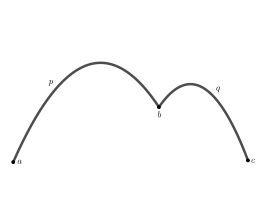
\includegraphics[trim=0.4cm 1.9cm 0.5cm 2.1cm, clip]{path_transitive}}
\end{center}
\caption{A path from $a$ to $c$.}
\label{F:path_transitive}
\end{figure}
%\includegraphics[trim=left bottom right top, clip]{file}

\begin{lemma}[The Gluing Lemma]\index{Gluing Lemma}  Let $A$ and $B$ be closed subsets of a space $X = A \cup B$, and let $f:A \to Y$ and $g: B \to Y$ be continuous functions into a space $Y$ such that $f(x)=g(x)$ for all $x \in (A \cap B)$. Then the function $h:X \to Y$ defined by 
\[h(x) = \begin{cases} f(x) &\text{ if } x \in A \\ g(x) &\text{ if } x \in B \end{cases}\]
is continuous. 
\end{lemma}

\begin{figure}[h]
\begin{center}
\resizebox{!}{2.0in}{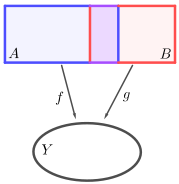
\includegraphics{Gluing_Lemma.eps}}
\end{center}
\caption{The Gluing Lemma.}
\label{F:Gluing_Lemma}
\end{figure}
%\includegraphics[trim=left bottom right top, clip]{file}

\begin{proof} Let $A$ and $B$ be closed subsets of a space $X = A \cup B$, and let $f:A \to Y$ and $g: B \to Y$ be continuous functions into a space $Y$ such that $f(x)=g(x)$ for all $x \in (A \cap B)$ as illustrated in Figure \ref{F:Gluing_Lemma}. Define $h: X \to Y$ by
\[h(x) = \begin{cases} f(x) &\text{ if } x \in A \\ g(x) &\text{ if } x \in B. \end{cases}\] 
To show that $h$ is continuous, let $C$ be a closed subset of $Y$. Then 
\[h^{-1}(C) = \{x \in X \mid h(x) \in C\} = \{x \in A \mid f(x) \in C\} \cup \{x \in B \mid g(x) \in C\} = f^{-1}(C) \cup g^{-1}(C).\]
Since $f$ is continuous, $f^{-1}(C)$ is closed in the subspace topology on $A$ and since $g$ is continuous $g^{-1}(C)$ is closed in the subspace topology on $B$. So $f^{-1}(C) = A \cap D$ and $g^{-1}(C) = B \cap E$ for some closed sets $D$ and $E$ of $X$. The fact that $A$ is closed in $X$ implies that $A \cap D$ is closed in $X$. Similarly, the fact that $B$ is closed in $X$ implies that $B \cap E$ is closed in $X$. Thus,
\[h^{-1}(C) = f^{-1}(C) \cup g^{-1}(C) = (A \cap D) \cup (B \cap E)\]
is a  finite union of closed sets in $X$ and so is closed in $X$. Since $h^{-1}(C)$ is closed for every closed set in $Y$, it follows that $h$ is continuous.
\end{proof}

We can use the Gluing Lemma to create a path from $a$ to $c$ given a path from $a$ to $b$ and a path from $b$ to $c$.

\begin{activity} Use the Gluing Lemma to explain why the path product given in the following definition is actually a path from $p(0)$ to $q(1)$. 

\begin{definition} Let $p$ be a path from $a$ to $b$ and $q$ a path from $b$ to $c$ in a space $X$. The \textbf{path product}\index{path product} $q*p$ is the path in $X$ defined by 
\[(q*p)(x) = \begin{cases} p(2x) &\text{ for } 0 \leq x \leq \frac{1}{2} \\ q(2x-1) &\text{ for } \frac{1}{2} \leq x \leq 1. \end{cases}\]
\end{definition}

\end{activity}

\begin{comment}

\ActivitySolution The Gluing Lemma allows us to piece together the paths $p$ and $q$. Let $A = \left[0 \frac{1}{2}\right]$, $B = \left[\frac{1}{2}, 1\right]$, $f(x) = p(2x)$, and $g(x) = q(2x-1)$. Then $A \cap B = \left\{\frac{1}{2} \right\}$. Note that $f\left(\frac{1}{2}\right) = p(1) = b = q(0) = g\left(\frac{1}{2}\right)$. It follows that $h$ as in the Gluing Lemma is a path from $a$ to $c$. 

\end{comment}

Now we can show that path connectedness defines an equivalence relation on a topological space. 

\begin{activity} Let $(X,\tau)$ be a topological space. Define a relation on $X$ as follows:
\begin{equation} \label{eq:path_equivalence}
a \sim b \text{ if there is a path in } X \text{ from } a \text{ to } b. 
\end{equation}
\ba
\item Explain why $\sim$ is a reflexive relation.

\item Explain why $\sim$ is a symmetric relation.

\item Explain why $\sim$ is a transitive relation.

\ea

\end{activity}

\begin{comment}

\ActivitySolution

\ba
\item Let $a \in X$. The constant function $p : [0,1] \to X$ defined by $p(x) = a$ for all $x in X$ is a path from $a$ to $a$. So $a \sim a$ and $\sim$ is a reflexive relation.

\item Let $b \in X$ such that $a \sim b$. Then there is a path $p:[0,1] \to X$ from $a$ to $b$. The function $q : [0,1] \to X$ defined by $q(x) = p(1-x)$ is a path from $b$ to $a$. So $b \sim a$ and $\sim$ is symmetric.

\item Assume $a \sim b$ and let $c \in X$ such that $b \sim c$. So there is a path $p$ from $a$ to $b$ and a path $q$ from $b$ to $c$. The path product $q*p$ is a path from $a$ to $c$, which makes $a \sim c$. We conclude that $\sim$ is transitive and an equivalence relation.

\ea

\end{comment}
 
Since $\sim$ as defined in (\ref{eq:path_equivalence}) is an equivalence relation, the relation partitions $X$ into a union of disjoint equivalence classes. The equivalence class of an element $[a]$ is called a \emph{path component} of $X$, and is the largest path connected subset of $X$ that contains $a$. 

\begin{definition} The \textbf{path component}\index{path component} of an element $a$ in a topological space $(X, \tau)$ is the largest path connected subset of $X$ that contains $a$. 
\end{definition}
 
\csection{Path Connectedness and Connectedness}

Path connectedness and connectedness are different concepts, but they are related. In this section we will show that any path connected space must also be connected. We will see later that the converse is not true except in finite topological spaces. 

\begin{theorem} \label{thm:pctoc} If a topological space $X$ is path connected, then $X$ is connected.
\end{theorem}
 
\begin{proof} Suppose that $X$ is path connected. Let $a \in X$ and for any $x \in X$ let $p_x$ be a path from $a$ to $x$. Let $C_x = p_x([0,1])$. Now $C_x$ is the continuous image of the connected set $[0,1]$ in $\R$, so $C_x$ is connected. Also, $p_x(0) = a \in C_x$ and $p_x(1) = x \in C_x$. Thus, every set $C_x$ contains $a$ and so $\bigcap_{x \in X} C_x$ is not empty. Therefore, 
\[C = \bigcup_{x \in X} C_x\]
is a connected subset of $X$. But every $x \in X$ is in a $C_x$, so $C = X$. We conclude that $X$ is connected. 
\end{proof}

In the following sections we explore the reverse implication in Theorem \ref{thm:pctoc} -- that is, does connectedness imply path connectedness. 

\csection{Path Connectedness and Connectedness in Finite Topological Spaces}

In this section we will demonstrate that connectedness and path connectedness are equivalent concepts in finite topological spaces. In the following section, we prove that path connectedness and connectedness are not equivalent in infinite topological spaces. Throughout this section, we assume that $X$ is a finite topological space. We begin with an example to motivate the main ideas. 

\begin{activity} \label{act:minimal_nbhds} Let $X = \{a,b,c,d\}$ and $\tau = \{\emptyset, \{b\}, \{c\}, \{a,b\}, \{b,c\}, \{a,b,c\}, \{b,c,d\}, X\}$. Assume that $\tau$ is a topology on $X$. 
\ba
\item Is $X$ connected? Explain.

\item For each $x \in X$, let $U_x$ be the intersection of all open sets that contain $x$ (we call $U_x$ a \emph{minimal neighborhood} of $x$). 

\begin{definition} \label{def:min_nghb} For $x \in X$, the \textbf{minimal neighborhood}\index{minimal neighborhood} $U_x$ of $x$ is the intersection of all open sets that contain $x$. 
\end{definition}

Find $U_x$ for each $x \in X$. 

\item We will see that the minimal neighborhoods of $X$ are path connected. Here we will illustrate with $U_d$. 

	\begin{enumerate}[i.] 
	\item Let $p : [0,1] \to X$ be defined by 
\[p(t) = \begin{cases} b &\text{if } 0 \leq t < \frac{1}{2} \\ d &\text{if } \frac{1}{2} \leq t \leq 1. \end{cases}\]
Show that $p$ is a path in $U_d$ from $b$ to $d$.

	\item Let $p : [0,1] \to X$ be defined by 
\[p(t) = \begin{cases} c &\text{if } 0 \leq t < \frac{1}{2} \\ d &\text{if } \frac{1}{2} \leq t \leq 1. \end{cases}\]
Show that $p$ is a path in $U_d$ from $c$ to $d$.

	\item Explain why $U_d$ is path connected.
	
	\end{enumerate} 

\ea

\end{activity}

\begin{comment}

\ActivitySolution

\ba
\item  The answer is yes. The only proper open set that contains $d$ is $\{b,c,d\}$, and $\{a\}$ is not an open set, so there is no pair of disjoint, non-empty open subsets of $X$ whose union is $X$. 

\item  The singleton sets $\{b\}$ and $\{c\}$ are open, so $U_b = \{b\}$ and $U_c = \{c\}$. We take each other element in turn:
\begin{itemize}
\item $U_a = \{a,b\} \cap \{a,b,c\} \cap X = \{a,b\}$,
\item $U_d = \{b,c,d\} \cap X = \{b,c, d\}$.
\end{itemize}
	\begin{enumerate}[i.] 	
	\item  We check the inverse images of each open set in $X$:
\begin{itemize}
\item $p^{-1}(\emptyset) = \emptyset$
\item $p^{-1}(\{b\}) = \left[0, \frac{1}{2}\right)$
\item $p^{-1}(\{c\}) \emptyset$
\item $p^{-1}(\{a,b\}) = \left[0, \frac{1}{2}\right)$
\item $p^{-1}(\{b,c\} = \left[0, \frac{1}{2}\right)$
\item $p^{-1}(\{a,b,c\}) = \left[0, \frac{1}{2}\right)$
\item $p^{-1}(\{b,c,d\}) = [0,1]$
\item $p^{-1}(X) = [0,1]$.
\end{itemize}
So $p^{-1}(O)$ is open for every open set $O$ in $X$. Therefore, $p$ is continuous. 

	\item  We check the inverse images of each open set in $X$:
\begin{itemize}
\item $p^{-1}(\emptyset) = \emptyset$
\item $p^{-1}(\{b\}) = \emptyset$
\item $p^{-1}(\{c\}) \left[0, \frac{1}{2}\right)$
\item $p^{-1}(\{a,b\}) = \emptyset$
\item $p^{-1}(\{b,c\} = \left[0, \frac{1}{2}\right)$
\item $p^{-1}(\{a,b,c\}) = \left[0, \frac{1}{2}\right)$
\item $p^{-1}(\{b,c,d\}) = [0,1]$
\item $p^{-1}(X) = [0,1]$.
\end{itemize}
So $p^{-1}(O)$ is open for every open set $O$ in $X$. Therefore, $p$ is continuous. 

	\item The answer is yes. The constant function from $[0,1]$ to $U_d$ defined by $p(x) = d$ for all $x \in [0,1]$ is a path from $d$ to $d$. There is a path $p_{bd}$ from $b$ to $d$ and a path $p_{cd}$ from $c$ to $d$. The function $p_{db}$ defined by $p_{db}(t) = p_{bd}(1-t)$ is a path from $d$ to $b$. The composite, $p_{db}p_{cd}$ is then a path from $c$ to $b$ and there is a path between any two points in $U_d$. We conclude that $U_d$ is path connected.  

	\end{enumerate}
\ea

\end{comment}

The terminology in Definition \ref{def:min_nghb} is apt. Since every neighborhood $N$ of a point $x \in X$ must contain an open set $O$ with $x \in O$, it follows that $U_x \subseteq O \subseteq N$. So every neighborhood of $x \in X$ has $U_x$ as a subset. In addition, when $X$ is finite, the set $U_x$ is a finite intersection of open sets, so the sets $U_x$ are open sets (this is not true in general in infinite topological spaces -- you should find an example where $U_x$ is not open). In Activity \ref{act:minimal_nbhds} we saw that $U_x$ was path connected for a particular $x$ in one example. The next activity shows that this result is true in general in finite topological spaces.

\begin{activity} Let $X$ be a finite topological space, and let $x \in X$. In this activity we demonstrate that $U_x$ is path connected. Let $y \in U_x$ and define $p : [0,1] \to X$ by 
\[p(t) = \begin{cases} y &\text{if } 0 \leq t < \frac{1}{2} \\ x &\text{if } \frac{1}{2} \leq t \leq 1. \end{cases}\]
To prove that $p$ is continuous, let $O$ be an open set in $X$. We either have $x \in O$ or $x \notin O$. 
\ba
\item Suppose $x \in O$. Why must $y$ also be in $O$? What, then, is $p^{-1}(O)$? 

\item Now suppose $x \notin O$. There are two cases to consider.
	\begin{enumerate}[i.]
	\item What is $p^{-1}(O)$ if $y \in O$?
		
	\item What is $p^{-1}(O)$ if $y \notin O$?
		
	\end{enumerate}

\item Explain why $p$ is a path from $y$ to $x$. 

\item Show that we can find a path between any two points in $U_x$. Conclude that $U_x$ is path connected.

\ea

\end{activity}

\begin{comment}

\ActivitySolution

\ba
\item Every open set containing $x$ contains $U_x$. Since $y \in U_x$, it follows that $y \in O$. Suppose $x \in O$. Why must $y$ also be in $O$? Since $p(t) \in O$ for every $t$ in $[0,1]$, we conclude that $p^{-1}(O) = [0,1]$.  

\item Now suppose $x \notin O$. 
	\begin{enumerate}[i.]
	\item If $y \in O$, then $p^{-1}(O) =  \left[0, \frac{1}{2}\right)$.
		
	\item If $y \notin O$, then $p^{-1}{O} =  \emptyset$.
		
	\end{enumerate}

\item So $p^{-1}(O)$ is open in $[0,1]$ for every open set $O$ in $X$. Therefore, $p$ is continuous and is a path from $y$ to $x$. 

\item We have seen that there is a path $p_{yx}$ from $y$ to $x$ for any $y \in U_x$. Let $a$ and $b$ be points  in $U_x$. There is a path $p_{ax}$ from $a$ to $x$ and a path $p_{bx}$ from $b$ to $x$. Since points being path connected is a symmetric relation, there is a path $p_{xb}$ from $x$ to $b$. Then path product $p_{xb}*p_{ax}$ is then a path from $a$ to $b$ in $U_x$. Since path-connectedness is reflexive and symmetric, we conclude that there is a path between any two points in $U_x$, so $U_x$ is a path connected set. 

\ea

\end{comment}

The sets $U_x$ collectively form the space $X$, and each of the $U_x$ is a path connected subspace. So every point in $X$ is contained in some neighborhood with a path connected subset containing $x$. Spaces with this property are called \emph{locally path connected}.

\begin{definition} A topological space $(X, \tau)$ is \textbf{locally path connected at } $x$ if every neighborhood of $x$ contains a path connected open neighborhood with $x$ as an element. The space $(X, \tau)$ is \textbf{locally path connected}\index{path connected!locally} if $X$ is locally path connected at every point.
\end{definition}

If $X$ is a finite topological space, for any $x \in X$ the set $U_x$ is the smallest open set containing $x$. This means that any neighborhood of $N$ of $x$ will contain $U_x$ as a subset. Thus, a finite topological space is locally path connected (this is not true in general of infinite topological spaces). One consequence of a locally path connected space is the following.

\begin{lemma} \label{lem:open_PC} A space $X$ is locally path connected if and only if for every open set $O$ of $X$, each path component of $O$ is open in $X$.
\end{lemma}

\begin{proof} Let $X$ be a locally path connected topological space. We first show that for every open set $O$ in $X$, every path component of $O$ is open in $X$. Let $O$ be an open set in $X$ and let $P$ be a path component of $O$. Let $p \in P$. Since $X$ is locally path connected, the neighborhood $O$ of $x$ contains an open path connected neighborhood $Q$ of $p$. The fact that $p \in Q$ and $P$ is a path component of $O$ implies that $Q \subseteq P$. Thus, $P$ contains a neighborhood of $p$ and $P$ is open. 

Now we show that if for every open set $O$ in $X$ the path components of $O$ are open in $X$, then $X$ is locally path connected. Let $x \in X$ and let $N$ be a neighborhood of $x$. Then $N$ contains an open set $U$ with $x \in U$. Let $P$ be the path component in $U$ that contains $x$. Now $P$ is path connected and, by hypothesis, $P$ is open in $X$ and so is an open path connected neighborhood of $x$. Thus, $N$ contains a path connected neighborhood of $x$ and $X$ is locally path connected at every point.

\end{proof}

Since $X$ is open in $X$ whenever $X$ is a topological space, a natural corollary of Lemma \ref{lem:open_PC} is the following.

\begin{corollary} Let $X$ be a locally path connected topological space. Then every path component of $X$ is open in $X$. 
\end{corollary}
 
Since there are only finitely many open sets in the finite space $X$, any arbitrary intersection of open sets in $X$ just reduces to a finite intersection. So the intersection of any collection of open sets in $X$ is again an open set in $X$. We will show that $X$ is a union of path connected components, which will ultimately allow us to prove that if $X$ is connected, then $X$ is also path connected. 

\begin{activity} Let $X$ be a locally path connected topological space. In this activity we will prove that the components and path components of $X$ are the same.
\ba
\item Let $x \in X$, and let $C$ be the component of $X$ containing $x$ and $P$ be the path component of $X$ containing $x$. Show that $P \subseteq C$. 

\item To complete the proof that $P = C$, proceed by contradiction and assume that $C \neq P$. Let $Q$ be the union of all path components of $X$ that are different from $P$ and that intersect $C$. Each such path component is connected, and is therefore a subset of $C$. So $C = P \cup Q$. Explain why $P$ and $Q$ form a separation of $C$. (Hint: How do we use the fact that $X$ is locally path connected?)

\ea

\end{activity}


\begin{comment}

\ActivitySolution

\ba
\item Since $P$ is path connected, Theorem \ref{thm:pctoc} shows that $P$ is connected. The fact that $C$ is the largest connected subset of $X$ containing $x$ implies that $P \subseteq C$.  

\item  Lemma \ref{lem:open_PC} shows that $P$ is an open set, and that $Q$ is an open set. Since path components are either equal or disjoint, we have that $P \cap Q = \emptyset$. Therefore, if $C \neq P$, then $P$ and $Q$ form a separation of $C$. This contradicts the fact that $C$ is connected. We conclude that $C = P$ and that the components and path components of $X$ are the same. 

\ea

\end{comment}

We can now complete our main result of this section.

\begin{theorem} Let $X$ be a finite topological space. Then $X$ is connected if and only if $X$ is path connected. 
\end{theorem}

\begin{proof} Let $X$ be a finite topological space. Theorem \ref{thm:pctoc} demonstrates that if $X$ is path connected, then $X$ is connected. For the reverse implication, assume that $X$ is path connected. Then $X$ is composed of a single path component, $P=X$. Since the path components and components of $X$ are the same, we conclude that $P= X$ is a component of $X$ and that $X$ is connected. 
\end{proof}


\csection{Path Connectedness and Connectedness in Infinite Topological Spaces}

Given that connectedness and path connectedness are equivalent in finite topological spaces, a reasonable question now is whether the converse of Theorem \ref{thm:pctoc} is true in arbitrary topological spaces. As we will see, the answer is no. To find a counterexample, we need to look in an infinite topological space. There are many examples, but a standard example to consider is the \emph{topologist's sine curve}\index{topologist's sine curve}. This curve $S$ is defined as the union of the sets
\[S_1 = \{(0,y) \mid -1 \leq y \leq 1\}  \ \text{ and } \ S_2 = \left\{ \left(x,\sin\left(\frac{1}{x}\right)\right) \Big| \ 0 < x \leq 1\right\}.\]
A picture of $S$ is shown in Figure \ref{F:T_sin}.  
\begin{figure}[h]
\begin{center}
\resizebox{!}{1.75in}{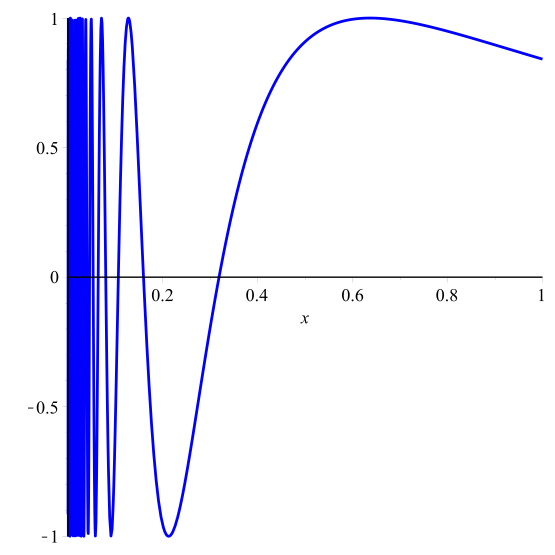
\includegraphics{T_sin}}
\end{center}
\caption{The topologist's sine curve.}
\label{F:T_sin}
\end{figure}



To understand if $S$ is connected, let us consider the relationship between $S$ and $S_2$. Figure \ref{F:T_sin} seems to indicate that $S = \overline{S_2}$. To see if this is true, let $q=(0,y) \in S_1$, and let $N$ be a neighborhood of $q$. Then there is an $\epsilon > 0$ such that $B = B(q, \epsilon) \subseteq N$. Choose $K \in \Z^+$ such that $\frac{1}{\arcsin(y)+2 \pi K} < \epsilon$, and let $z = \frac{1}{\arcsin(y)+2 \pi K}$. Then
\begin{align*}
d_E\left(q,\left(z, \sin\left(\frac{1}{z}\right)\right)\right) &=  d_E\left((0,y),(z, \sin(\arcsin(y)+2 \pi K)\right) \\
	&= d_E((0,y), (z,\sin(\arcsin(y)))) \\
	&= d_E((0,y), (z,y)) \\
	&= \la z \ra \\
	&< \epsilon,
	\end{align*}
and so $\left(z, \arcsin(z)\right) \in B(q, \epsilon)$ and every neighborhood of $q$ contains a point in $S_2$. Therefore, $S_1 \subseteq S_2' \subseteq \overline{S_2}$ and $\overline{S_2} = S$ in $S$.  The fact that $S$ is connected follows from Theorem \ref{thm:connected_limitpoints}. 

Now that we know that $S$ is connected, the following theorem demonstrates that $S$ is a connected space that is not path connected. 

\begin{theorem} The topologist's sine curve is connected but not path connected. 
\end{theorem}

\begin{proof} We know that $S$ is connected, so it remains to show that $S$ is not path connected. The sets $S_1$ and $S_2$ are connected (as continuous images of the interval $[0,1]$ and $(0,1]$, respectively). We will prove that there is no path $p$ in $S$ from $p(0) = (0,0)$ to $p(1) =  b$ for any point $b \in S_2$ by contradiction. Assume the existence of such a path $p$. Let $U = p^{-1}(S_1)$ and $V = p^{-1}(S_2)$. Then
\begin{equation} \label{eq:TSC_1}
[0,1] = p^{-1}(S) = p^{-1}(S_1 \cup S_2) = p^{-1}(S_1) \cup p^{-1}(S_2) = U \cup V.
\end{equation}
Note that $S_2$ is an open subset of $S$, since $S_2 = \left( \bigcup_{z = (x,y) \in S_2} B\left(z, \frac{x}{2}\right)\right) \cap S$. So the continuity of $p$ implies that $V$ is an open subset of $[0,1]$. Also, the fact that $p(0) \in S_1$ means that $U \neq \emptyset$, and the fact that $p(1) \in S_2$ means that $V \neq \emptyset$. If we demonstrate that $U$ is an open subset of $[0,1]$, then Equation (\ref{eq:TSC_1}) will imply that $[0,1]$ is not connected, a contradiction. So we proceed to prove that $U$ is open in $[0,1]$.

Let $x \in U$, and so $p(x)$ in $S_1$. The set $O = B_S\left(p(x), \frac{1}{2}\right) \cap S$ is open in $S$. The continuity of $p$ then tells us that $p^{-1}(O)$ is open in $[0,1]$. So there is a $\delta > 0$ such that the open ball $B=B_{[0,1]}(x, \delta)$ is a subset of $p^{-1}(O)$. We will prove that $p(B) \subseteq S_1$. This will imply that $B \subseteq U$ and so $U$ is a neighborhood of each of its points, and $U$ is therefore an open set. 

\begin{figure}[h]
\begin{center}
\resizebox{!}{2.25in}{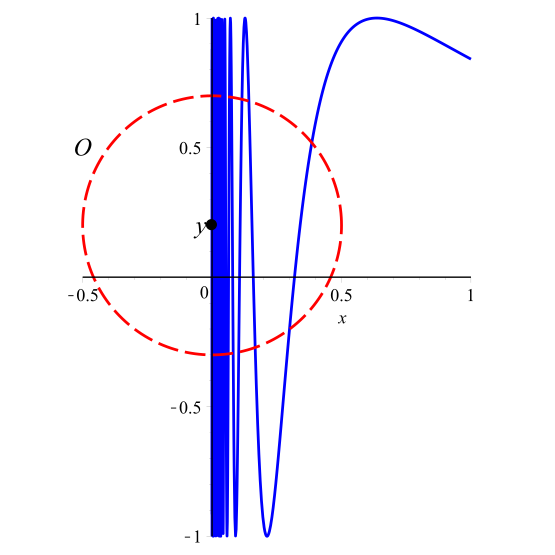
\includegraphics{O_set}}
\end{center}
\caption{The set $O$.}
\label{F:TSC_O}
\end{figure}
Every element in $B$ is mapped into $O$ by the path $p$. The set $O$ is complicated, consisting of infinitely many sub-curves of the curve $S_2$, along with points in $S_1$, as illustrated in Figure \ref{F:TSC_O}. To simplify our analysis, let us consider the projection onto the $x$-axis. The function $P_x : \R^2 \to \R$ defined by $P_x(x,y) = x$ is a continuous function. Let $I = P_x(p(B))$. Since $p(B) \subseteq O$, we know that $I \subseteq P_x(O)$. Let $Z = P_x(O)$. So $I \subseteq Z$. Since $B$ is a connected set ($B$ is an interval), we know that $p(B)$ is a connected set. The fact that $P_x$ is continuous means that $I = P_x(p(B))$ is connected as well. Now $I$ is a bounded subset of $\R$, so $I$ must be a bounded interval. Recall that $x \in B$ and so $p(x) \in p(B)$. The fact that $p(x) \in S_1$ tells us that $0 = P_x(p(x)) \in P_x(p(B)) = I$. So $I \neq \emptyset$. There are two possibilities for $I$: either $I = \{0\}$, or $I$ is an interval of positive length. We consider the cases.

Suppose $I = \{0\}$. Then the projection of $p(B)$ onto the $x$-axis is the single point $0$ and $p(B) \subseteq S_1$ as desired. Suppose that $I$ is an interval of the form $[0,d]$ or $[0,d)$ for some positive number $d$. The structure of $O$ would indicate that there must be some gaps in the set $Z$, the projection of $O$ onto the $x$-axis. This implies that $I$ cannot be a connected interval. We proceed to show this. In other words, we will prove that $I \setminus Z \neq \emptyset$ (which is impossible since $I \subseteq Z$). Remember that $p(x) \in S_1$, so let $p(x) = (0, q)$. We consider what happens if $q < \frac{1}{2}$ and when $q \geq \frac{1}{2}$.  

Suppose $q < \frac{1}{2}$. Then the ball $B_S\left(p(x), \frac{1}{2}\right)$ contains only points with $y$ value less than 1. Let $N \in \Z^+$ so that $t=\frac{1}{\pi/2+2N\pi} < d$. Then $t \in I$. But $\sin\left(\frac{1}{t}\right) = \sin(\pi/2 + 2N\pi) = \sin(\pi/2) = 1$, and so $\left(t,\sin\left(\frac{1}{t}\right)\right)$ is not in $O$. Thus, $t \notin Z$. Thus we have found a point in $I \setminus Z$. 

Finally, suppose $q \geq \frac{1}{2}$. Then the ball $B_S\left(p(x), \frac{1}{2}\right)$ contains only points with $y$ value greater than $-1$. Let $N \in \Z^+$ so that $t=\frac{1}{3\pi/2+2N\pi} < d$. Then $t \in I$. But $\sin\left(\frac{1}{t}\right) = \sin(3\pi/2 + 2N\pi) = \sin(3\pi/2) = -1$, and so $t \notin Z$. Thus we have found a point in $I \setminus Z$. 

We conclude that there can be no path in $S$ from $(0,0)$ to any point in $S_2$, completing our proof that $S$ is not path connected. (In fact, the  argument given shows that there is no path in $S$ from any point in $S_1$ to any point in $S_2$. 
\end{proof}

\csection{Summary}
Important ideas that we discussed in this section include the following.
\begin{itemize}
\item A path in a topological space $X$ is a continuous function $p$ from the interval $[0,1]$ to $X$. If $p(0) = a$ and $p(1) = b$, then $p$ is a path from $a$ to $b$. 
\item A subspace $A$ of a topological space $X$ is path connected if, given any $a, b \in A$ there is a path in $A$ from $a$ to $b$.
\item The path component of an element $a$ in a topological space $(X, \tau)$ is the largest path connected subset of $X$ that contains $a$. 
\item A topological space $(X, \tau)$ is locally path connected at $x$ if every neighborhood of $x$ contains a path connected subset with $x$ as an element. The space $(X, \tau)$ is locally path connected if $X$ is locally path connected at every point.
\item Connectedness and path connectedness are equivalent in finite topological spaces, and path connectedness implies connectedness in general. However, there are topological spaces that are connected but not path connected. One example is the topologist's sine curve. 
\end{itemize}


\csection{Exercises}

\be

\item Let $X$ be a topological space and for each $x \in X$ let $PC(x)$ denote the path component of $x$. Prove the following.

\ba

\item If $A$ is a path connected subset of $X$, then $A \subseteq PC(x)$ for some $x \in X$.

\item The space $X$ is path connected if and only if $X = PC(x)$ for some $x \in X$.

\ea

\begin{comment}

\ExerciseSolution

\ba

\item Let $A$ be a path connected subset of $X$, and let $x \in A$. Since $PC(x)$ is the largest path connected subset of $X$ that contains $x$, it follows that $A \subseteq PC(x)$.

\item Suppose that $X$ is path connected. Then $X$ is a path connected subset of $X$, so part (a) shows that $X = PC(x)$ for some $x \in X$. Conversely, if $X = PC(x)$ for some $x \in X$, then $X$ is path connected since $PC(x)$ is path connected.

\ea


\end{comment}

\item In Activity \ref{act:connected_compenent} of Section \ref{sec:Connected_topology} we showed that an arbitrary union of connected sets is connected provided the intersection of those sets is not empty. Is the same result true for path connected sets. That is, if $X$ is a topological space and $\{A_{\alpha}\}$ for $\alpha$ in some indexing set $I$ is a collection of path connected subsets of $X$ and $\bigcap_{\alpha \in I} A_{\alpha} \neq \emptyset$, must it be the case that $A = \bigcup_{\alpha \in I} A_{\alpha}$ is path connected? Prove your answer. 

\begin{comment}

\ExerciseSolution Suppose $\{A_{\alpha}\}$ for $\alpha$ in some indexing set $I$ is a collection of path connected subsets of $X$ such that $\bigcap_{\alpha \in I} A_{\alpha} \neq \emptyset$. Let $A = \bigcup_{\alpha \in I} A_{\alpha}$ and let $x, y \in A$. If $x$ and $y$ are both in $A_{\alpha}$ for some $\alpha \in I$, then the fact that $A_{\alpha}$ is path connected implies that there is a path between $x$ and $y$. So suppose, without loss of generality, that $x \in A_{\beta}$ and $y \in A_{\gamma}$ for some $\beta \neq \gamma$ in $I$. Let $z \in \bigcap_{\alpha \in I} A_{\alpha}$. The fact that $z \in A_{\beta}$ implies that there is a path in $A_{\beta}$ from $x$ to $z$. Also, $z \in A_{\gamma}$ so there is a path in $A_{\gamma}$ from $z$ to $y$. By transitivity, there is a path in $A$ from $x$ to $y$ and so $A$ is path connected. 

\end{comment}


\item \label{ex:PC_harmonic_broom} Let $X$ be the subspace of $(\R^2, d_E)$ consisting of the line segments joining the point $(0,1)$ to every point in the set $\left\{\left(\frac{1}{n}, 0\right) \mid n \in \Z^+\right\}$ as illustrated in Figure \ref{F:harmonic_broom}. This space is called the \emph{harmonic broom}.  
\begin{figure}[h]
\begin{center}
\resizebox{!}{1.75in}{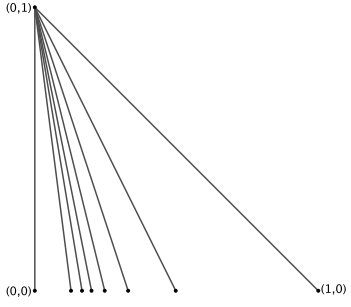
\includegraphics{Harmonic_broom.eps}}
\end{center}
\caption{The harmonic broom.}
\label{F:harmonic_broom}
\end{figure}
\ba

\item Show that the harmonic broom is connected.

\item Show that the harmonic broom is path connected.

\item Show that the harmonic broom is not locally connected. 

\item Show that the harmonic broom is not locally path connected. So path connectedness does not imply local path connectedness. 

\ea

\begin{comment}

\ExerciseSolution

\ba

\item We will show that the harmonic broom is path connected in part (b), and every path connected space is connected.

\item Let $p$ be a point in $X$, then the line segment containing the origin $o$ an $p$ provides a path from $o$ to $p$. So if $p$ and $q$ are in $X$, there is a path from $p$ to $o$, and a path from $o$ to $q$. The path product then gives a path from $p$ to $q$. So $X$ is path connected. 

\item Let $o = (0,0)$ and let $B = B(o,0.5) \cap X$. Then $B$ is an open set in $X$ that contains $o$, but $B$ does not contain $(0,1)$. Note that any open subset of $B$ will contain infinitely many portions of segments from the point $(1,0)$ to points of the form $(a,0)$ for small enough values of $a$. These segments are not connected, and so $X$ is not locally connected. 

\item Again let $o = (0,0)$ and consider $V = B(o,0.5)$ as an open subset of $X$. Any open subset $U$ of $V$ that contains $o$ must contain an open ball of the form $B(o,r)$ for some $r > 0$. Let $n \in \Z^+$ such that $\frac{1}{n} < r$. Then $p = \left(\frac{1}{n}, 0\right)$ is in $B(o,r)$, but since $(0,1)$ is not in $V$ there is no path in $V$ from $p$ to $o$. So $X$ is not locally path connected. 

\ea

\end{comment}

\item In Exercise \ref{ex:PC_harmonic_broom} we see an example of a space that is path connected but not locally path connected. Is it possible to find a space that is locally path connected but not path connected? Verify your answer.

\begin{comment}

\ExerciseSolution The answer is yes. Let $X = (0,1) \cup (1,2)$ in $(\R^2, d_E)$. Since there is no path in $X$ from $0.5$ to $1.5)$, we see that $X$ is not path connected. However, if $x \in X$, then $x \in (0,1)$ or $x \in (1,2)$. But both $(0,1)$ and $(1,2)$ are path connected, so $X$ is locally path connected.

\end{comment}


\item We know that a space can be connected but not path connected. We also know that local path connectedness does not imply connectedness. However, if we combine these conditions then a space must be path connected. That is, show that if a topological space $X$ is connected and locally path connected, then $X$ is path connected. 

\begin{comment}

\ExerciseSolution Let $X$ be a topological space that is connected and locally path connected. We know that $X$ can be written as a disjoint union of path components. That is $X = \bigcup_{\alpha \in I} P_{\alpha}$, where $P_{\alpha}$ are the distinct path components in $X$ for $\alpha$ in some indexing set $I$. Since $X$ is locally path connected, we know that each $P_{\alpha}$ is and open set. So if there is more than one path component, say $P_{\alpha}$ and $P_{\beta}$, then $P_{\alpha}$ and $\bigcup_{\substack{\gamma \in I \\ \gamma \neq \alpha}} P_{\gamma}$ form a separation of $X$. But this is impossible if $X$ is connected, so we conclude that there is only one path component in $X$ and $X$ is path connected. 

\end{comment}


\item Let $X$ be a nonempty set and let $p$ be a fixed element in $X$. Let $\tau_p$ be the particular point topology and $\tau_{\overline{p}}$ the excluded point topology on $X$. That is
\begin{itemize}
\item $\tau_{p}$ is the collection of subsets of $X$ consisting of $\emptyset$, $X$, and all of the subsets of $X$ that contain $p$.  
\item $\tau_{\overline{p}}$ is the collection of subsets of $X$ consisting of $\emptyset$, $X$, and all of the subsets of $X$ that do not contain $p$. 
\end{itemize}
That the particular point and excluded point topologies are topologies is the subject of Exercises (\ref{ex:particular_point_topology}) and (\ref{ex:excluded_point_topology}) on page \pageref{ex:particular_point_topology}. 

Determine, with proof, the path connected subsets of $X$ when 
\ba
\item $X$ has the particular point topology $\tau_p$

\item $X$ has the excluded point topology $\tau_{\overline{p}}$. 

\ea

\begin{comment}

\ExerciseSolution

 	\ba
	\item Let $C$ be a subset of $X$. We will show that $C$ is path connected if and only if $p \in C$. First we show that for any $y \in X$ there is a path in $X$ from $p$ to $y$. Let $y \in X$. Define $q: [0,1] \to X$ by 
	\[q(x) = \begin{cases} p &\text{ if } 0 \leq x < 1 \\ y & \text{ if } x = 1. \end{cases}\]
	Let $O$ be an open set in $(X, \tau_{p})$. If $O = \emptyset$, then $q^{-1}(O) = \emptyset$, which is open. If $O \neq \emptyset$, then $O$ contains $p$. We consider the cases where $y \in O$ or $y \notin O$. 
	\begin{itemize}
	\item If $y \in O$, then $q^{-1}(O) = [0,1]$, which is open in $[0,1]$. 
	\item If $y \notin O$, then $q^{-1}(O) = [0,1)$, which is also open in $[0,1]$. 
	\end{itemize}
In either case, $q^{-1}(O)$ is open and so there is a path from $p$ to $y$ for any $y \in X$. 

Now let $b, c \in C$. We just showed that there is a path from $p$ to $c$ and a path from $p$ to $b$. Path connectedness is symmetric and transitive, so there is a path from $c$ to $b$. Thus, $C$ is path connected. 

Finally, suppose $p \notin C$. Let $C_0$ be a subset of $C$. Then $C_0 \cup \{p\}$ is an open set in $X$ and $C \cap (C_0 \cup \{p\}) = C_0$. So the subspace topology on $C$ is the discrete topology. It follows that $C$ is disconnected. Since path connectedness implies connectedness, we conclude that $C$ is not path connected. 
	
	\item  We make a similar argument as in part (a). Let $y \in X$. and define $q:[0,1] \to X$ by 
\[q(x) = \begin{cases} p &\text{ if } x=0 \\ y & \text{ if } 0 < x \leq 1. \end{cases}\]
	Let $O$ be an open set in $(X, \tau_{\overline{p}})$. If $O = \emptyset$, then $q^{-1}(O) = \emptyset$ which is open. Suppose $O \neq \emptyset$. Since $O$ is open, we know that $O$ does not contain $p$. We consider the cases where $y \in O$ or $y \notin O$. 
	\begin{itemize}
	\item If $y \in O$, then $q^{-1}(O) = (0,1]$, which is open in $[0,1]$. 
	\item If $b \notin O$, then $q^{-1}(O) = \emptyset$, which is also open in $[0,1]$. 
	\end{itemize}
In either case, $q^{-1}(O)$ is open and so there is a path from $p$ to $y$ for any $y \in X$. Again, by symmetry, there is also a path from $z$ to $p$ for any $z \in X$.  Thus, given any elements $a$ and $b$ in $X$, there is a path from $a$ to $b$. 

Let $C$ be a nonempty subset of $X$ with $p \in C$. The previous argument shows that $C$ is path connected. 

Now suppose $p \notin C$. Then every subset of $C$ is an open set and the subspace topology on $C$ is the discrete topology. It follows that $C$ is disconnected and is not path connected. 
	
	\ea


\end{comment}


\item For each of the following, answer true if the statement is always true. If the statement is only sometimes true or never true, answer false and provide a concrete example to illustrate that the statement is false. If a statement is true, explain why. 
\ba

\item If $X$ is a path connected topological space, then any subspace of $X$ is path connected. 
	
\item If $A$ and $B$ are path connected subspaces of a topological space $X$, then $A \cap B$ is path connected. 

\item There is no path from $a$ to $b$ in $(X, \tau)$, where $\tau$ is the discrete topology.

\item If $X$ is a compact locally path connected topological space, then $X$ has only finitely many path components. 

\item Every locally path connected space is locally connected. 


	\ea

\begin{comment}

\ExerciseSolution

\ba

\item This statement is false. Let $X = (0,2)$ with the Euclidean metric topology. Then $X$ is path connected. However, there is no path between $0.5$ and $0.75$ in the subspace $(0,0.5] \cup [0.75, 2)$. 

\item This statement is false. Let $A$ be the top half of the circle $x^2+y^2 = 1$ and $B = \{(x,0) \mid -1 \leq x \leq 1\}$ in $\R^2$ with the Euclidean metric topology. Then any two points in $A$ can be connected with an arc, and $B$ is an interval, so both $A$ and $B$ are connected. However, $A \cap B = \{(-1,0), (1,0)\}$ and there is no path between $(-1,0)$ and $(1,0)$ in $A \cap B$. 

\item This statement is false. Suppose $p$ is a path from $a$ to $b$ in $(X, \tau)$, where $\tau$ is the discrete topology. Then $p^{-1}(\{a\})$ and $p^{-1}(\{b\})$ must be non-empty and open in $[0,1]$. It follows that 
\[[0,1] = p^{-1}(X) = p^{-1}(\{a\} \cup \{b\}) = p^{-1}(\{a\}) \cup p^{-1}(\{b\}).\]
Since no element in $[0,1]$ can map to both $a$ and $b$, the fact that $p^{-1}(\{a\}) \cap p^{-1}(\{b\}) = \emptyset$ implies that $[0,1]$ is disconnected. So there is no path from $a$ to $b$ in $X$ with the discrete topology.

\item This statement is true. Let $\{P_{\alpha}\}_{\alpha \in I}$ be the collection of distinct path components in $X$. Since $X$ is locally path connected, each path component is open in $X$. So $\bigcup_{\alpha \in I} P_{\alpha}$ is an open cover of $X$ and so has a finite subcover $\{P_{\alpha_1}, P_{\alpha_2}, \ldots, P_{\alpha_m}\}$. But the $P_{\alpha_i}$ are disjoint, so no set can be removed from this collection and still have a cover. So $X$ has exactly $m$ path components. 

\item This statement is true. Let $X$ be a locally path connected space. We will show that $X$ is locally connected. Let $x \in X$ and let $N$ be a neighborhood of $x$. Since $X$ is locally path connected, there exists an open path connected neighborhood $U$ of $x$ contained in $N$. But path connectedness implies connectedness, so $U$ is an open connected neighborhood of $x$. It follows that $X$ is locally connected. 


\ea


\end{comment}

\ee

